%===================================== CHAP 3 =================================

\chapter{Related Work}

Recent advances in deep learning may render several state-of-the-art approaches within other fields of artificial intelligence (AI) such as image classification and natural language processing obsolete, as they have been outperformed by more generally applicable algorithms of deep learning \citep{LeCun2015, Schmidhuber2014}. These advances are due to both computational as well as algorithmic improvements within the field. New insights into how high-level cognition may be constituted and emerge in neural networks may further advance the field's capabilities, possibly beyond what can be achieved only by an increase in computational power. At the very core of such new insights lies the ability for abstraction and generalisation in neural networks. These aspects have been addressed by authors such as \cite{McClelland1995}, and more recently \cite{Hattori2014}. In their seminal paper, \cite{McClelland1995} propose a dual-network memory architecture, hypothesising that the brain solves the problem of long-term memory and memory consolidation by the use of a dual-network memory architecture. Because the body of research on artificial dual-network memory models is fairly limited, the goal of this thesis is to further investigate issues such as catastrophic forgetting and generalisation in that context. Catastrophic forgetting is of central importance to memory formation in neural networks, and avoiding it is crucial to forming certain representations from different types of patterns and memory. Elucidating questions related to abstraction in this architecture could provide key insights for further advances within deep learning, artificial intelligence, neuroscience and psychology. Furthermore, the long-standing symbol grounding problem is addressed by authors such as \cite{Yamashita2008, Tani2014}, who propose solutions to this long standing problem. However, their models are still entirely domain-specific. Therefore I wish to investigate the potential for combining their models with the model of \citep{Hattori2014} in my future work.
In order to investigate the body of research on the topic, the databases of Scopus, Web of Science, IEEE, Nature, those indexed in Mendeley, and arXiv were used to locate references of interest. Furthermore, a process of following networks of citations was employed, particularly by considering the paper \citep{McClelland1995}. Furthermore, as some heavily cited authors appeared, such as Tani, LeCun, Bengio, and Schmidhuber, their lists of publications were used as sources for further extending the bibliography. Note that as there is a significant time limit posed on this thesis, the scope of the literary review has to be reduced accordingly. It is, nevertheless, my view that a sufficient overview of relevant articles related to the thesis topic is presented, forming a foundation for the discussion of the thesis findings, as well as for future work that I wish to pursue (outlined in chapter \ref{chpt:discussion_future_work}).

% =================================================================================================
\section{The Dual-network Memory Architecture}

In this seminal paper, \cite{McClelland1995} propose a dual-network memory architecture in which the hippocampus is responsible for the consolidation of memories to the neocortex, with the neocortex storing semantic and episodic memory. The synthesis of recall from the deeper layers of the neocortex and representations in the working memory itself enables contexts to be distinguished or connected in the proposed model. The learning and consolidation to the neocortical module is essentially performed in an interleaved fashion; slowly potentiating and instantiating the memories from the hippocampal to the neocortical network. An approach closely resembling a bottom-up and top-down synthesis, where recall is combined with novel patterns. This raises the question of how such an interconnectedness is constituted both topologically speaking, as well as in terms of local information-processing. Furthermore, the question is whether principles from the environment of the neocortex and hippocampus need to be extracted and implemented to successfully have this functionality emerge in computational models, i.e. whether a synthesis of brain functionality constituted by additional parts would be crucial in regard to memory consolidation in the artificial model. For instance for the successful integration across memories. The proposed model of \citep{McClelland1995} suggests that the hippocampus and neocortex constitute the mechanisms for successful integration across memories, as well as keeping memories fairly intact. The specifics on how these mechanisms are constituted, however, remain obscure or undiscovered. This constitutes a core inspiration and foundation for an artificial neural network (ANN) model in this thesis. More specifically it lays out the foundation for investigating long-term memory and memory consolidation, by which I hope to attain more insight into mechanisms that enable generalisability and plasticity in ANN models.

\cite{McClelland1995} propose in their seminal paper a dual-network memory model which largely ameliorates the problem of catastrophic forgetting in ANNs, outperforming other algorithms of the time by far. However, work on this model is fairly limited, and it is with the aim of further extending the architecture that I regard one of the latest implementations of it, being the model of \cite{Hattori2014}. \cite{Hattori2010} proposes a model which fundamentally differs from the former implementations of \cite{French1997} and \cite{Ans1997} in that the hippocampal module is constituted by a chaotic neural network. Keep in mind that the phrases of hippocampal and neocortical networks should only be considered as borrowed terms for symbolising the networks of the model. The model networks are only very loosely coupled to biological functioning, with the approach outlined being only inspired by it.

\citep{French1997} propose a series of experiments that address the sensitivity-stability dilemma \citep{Hebb1949}, in which the authors demonstrate that a pseudo-recurrent network model performs significantly better than traditional feed-forwad back-propagate networks, mainly inspired by \cite{McClelland1995}. Different experiments are used to illuminate several aspects of the pseudo-recurrent network model. The key finding is that pseudo-recurrent networks using pseudo-patterns perform significantly better in terms of less catastrophic forgetting, suggesting that the brain may perform a type of pseudo-pattern compression and storage of information, too. Another point worth noting is that the networks that are simulated are of a fairly small scale, making them generalisable only to a certain extent due to network capacity. This seems to have been largely ignored by the authors. Therefore it would be interesting to look at the implications of both increasing the complexity as well as the scale of the network, such as in the models of \citep{Hattori2010, Hattori2014}. Note that the semi-distributedness of this paper's model arises naturally from the pseudo-recurrent neural network, as opposed to in the former papers of \cite{French1992, French1994}. This may suggest that the mechanism, which acts as an auto-associative memory, may also act as a predictor. In addition to completing incomplete, partial or fuzzy memories and retrieving them, it might therefore also provide a mechanism to filling in a story, or even imagining a story, creating it on the go by using the pseudo-recurrent mechanisms. This could suggest that the interleaving of memories in a pseudo-recurrent manner is at the heart of creativity, prediction and not the least; cognition. In relation to the thesis, I wish to investigate various successful or partly successful approaches for addressing convergence in the dual-network memory architecture. A key finding is that of pseudo-recurrency performing a crucial mechanism in interleaving and pattern generation. This may form a foundation for a comparative analysis in my future work, as well as providing insights into some underlying principles for the emergence of such mechanisms.

\cite{French2001} address the issues of the dual-network memory models in \citep{French1997, Ans1997}, illuminating key issues related to episodic memory, contextualisation, and pseudo-pattern generation and optimisation. In doing this, they conclude that the brain is likely to perform some kind of pseudo-pattern optimisation. Possibly in a stochastic way relative to how well it evaluates its performance and understanding of a currently perceived concept or state. When it comes to episodic memory, the work of \cite{Ans2000} is elaborated on, in which only dissimilar pseudo-inputs were used for consolidation to a neocortical network. Results demonstrated that the model was capable of generalising to and thus learning all patterns (20 patterns, where only 13 were explicitly taught to the neocortical network). This strengthens the view that a dual-network memory model is crucial for successful integration across memories. Another aspect that is addressed is contextualisation in the dual-network memory architecture. \cite{Ans2000} demonstrated that their implementation of a dual-network memory model performed better with pseudo-patterns with random initial input rather than when retrieving similar patterns from the neocortical module. This does pose an inconsistency both biologically and algorithmically speaking, because it is biologically implausible to retrieve an output representing the activity of the entire neocortical network, and algorithmically inefficient or possibly intractable with increasing network size, in order to interleave new memories with old. Furthermore, retrieving similar patterns mostly leads to a failure of convergence. This suggests that there may in fact be other, or more, principles that play a crucial role in the dual-network memory architecture. Summarising; the dual-network memory model offers significant benefits and advances in neural network models, but there seems to be an oversimplification related to pseudo-pattern formation and generation, affecting the integration across similar, yet separate memories. This is an aspect which I wish to further investigate in this thesis.

In this excellent paper, \cite{Hattori2014} presents a novel ANN model based on the dual-memory architecture of \cite{McClelland1995}. \cite{Hattori2014} demonstrates in several experiments that catastrophic forgetting is reduced to a large extent in the new model, and furthermore that it is superior to the dual-network memory architecture of \cite{Ans1997, French1997, Hattori2010}. \cite{Hattori2014} further demonstrates that the hippocampal network is capable of acquiring information rapidly, consolidating this to the neocortical network when it is successfully extracted in the HPC module.
However, the model is still not used to solve complex tasks, as the model is rather heavy in terms of computational complexity due to introducing more complex neuronal dynamics. The hippocampal network consists of McCulloch \& Pitts neurons, using the Oja rule for learning and updating connections between the different sub-modules, except for in the CA3 sub-module, where Hebbian learning with forgetting is used.
As for his experiments and results, he finds that mean goodness and perfect recall is worse in the hetero-associative case when compared to the auto-associative for the model. This may suggest that a significant amount of plasticity is missing in the model. This is further supported by the observation that a much higher turnover-rate than observed biologically speaking has to be employed for tuning the model. Looking to complex systems theory, some noise or chaos is required to arrive at a phase-transition between regular and chaotic dynamics, i.e. the critical phase, in which learning is made possible and efficient, \cite{Langton1990, Newman2003}. By using a very high neuronal turnover in the model, this suggests that the high turnover rate could be what alleviates the lack of plasticity in the proposed model. Despite improving training performance and pattern extraction, using too high a turnover-rate may also introduce too much randomness, rendering the representations too coarse-grained. Therefore it would be interesting to see parameter adjustments for the hetero-associative case in the hippocampal module, as this may pose different constraints on the network. Particularly an analysis of the edge of chaos for the CA3-part is something which I wish to further investigate in my future work. Another important aspect would be attempting to temporally extend the model, in an attempt to capture how episodic memory may be constituted in a complementary memory model. Such a synthesis could potentially introduce novel aspects of high-level cognition. It is therefore my aim in this thesis to look at variations in neuronal dynamics as well as topologies in a novel dual-network memory architecture, first by introducing a novel neocortical network.

\subsection{The Neocortical Module}

\cite{Hattori2010} trains the neocortical module using pseudo-patterns. A pseudo-pattern is a pattern representing the weighting and internal dynamics of a network. In his paper, \cite{Hattori2010} looks at two types of pseudo-patterns, which he refers to as type I and II. Type I is constructed in a very simple way: A random input is presented to the neocortical network, and the output is retrieved. This is then stored as an input-output pattern, called a pseudo-pattern of type I.

pseudo-patterns of type II are constructed in a slightly different manner, the approach being as follows:

\begin{enumerate}
\item Retrieve an extracted pattern from the hippocampal network.
\item For each element of the pattern, reverse is with a probability $p_r$.
\item Present the pattern to the neocortical network, and store the retrieved input-output pair (pseudo-pattern II) in a set.
\item Repeat step 2. and 3. until a certain number of pseudo-patterns of type II are obtained.
\end{enumerate}
Performing steps 1.-4. above results in a set of pseudo-patterns of type II.

After pseudo-patterns have been obtained, the neocortical network is simply trained on them by using FFBP, i.e. standard gradient-descent in weight space as outlined in \ref{BP}. Note that due to the nature of the pseudo-patterns, old memories are actually interleaved with old. This may be seen by considering that pseudo-pattern I is in fact the output obtained by presenting a random input to the network, the output reflecting a compressed version of the network weights at the time. When the network is trained on the pseudo-pattern along with a hippocampal pseudo-pattern, BP attempts to minimise the error between the old configuration of weights and the new hippocampal pseudo-pattern. Thus interleaving the old representation of memories with the new memory. In fact, \cite{Hattori2014} uses the exact same type of mechanisms for memory consolidation to the neocortical network.
Similarly, for a set of pseudo-patterns II, as elements are reversed in the hippocampal pseudo-pattern, the resulting pseudo-patterns II reflect both the network configuration (weights) and the novel hippocampal pseudo-pattern. This is a more explicit type of interleaving, where a new pattern which is to be learned is slightly randomized, creating a set of patterns which will reflect both the new memory as well as the old.

Memory recall in the neocortical network may be performed by presenting input patterns to the neocortical network and obtaining the resulting output from the network. Note that as outlined above, the neocortical network only learns the pseudo-patterns that are extracted by the hippocampal network. Therefore, some success criteria such as perfect recall depends strongly on the perfect extraction rate of the hippocampal network (i.e. when every part of the pattern has been successfully learned).

% ====================================
\subsection{The Hippocampal Module}
\subsubsection{\cite{Hattori2010}}
\begin{figure}
\centering
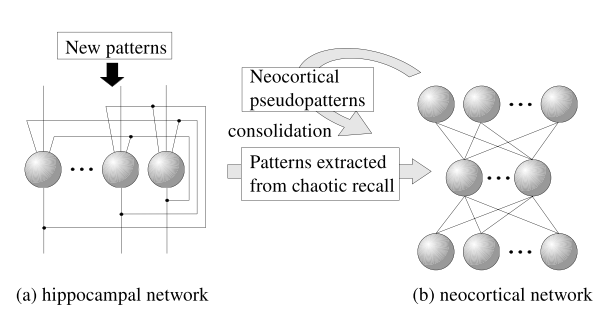
\includegraphics[width=10cm]{fig/hattori2010_model_structure}
\caption{An illustration from the paper of \cite{Hattori2010} of the proposed model. (a) represents the hippocampal module, whereas (b) represents the neocortical module. Note that the hippocampal module implements a Hopfield network, from which seemingly chaotic behaviour emerges when combined with the neuronal dynamics.}
\label{fig:hattori2010_model_structure}
\end{figure}

As can be seen from figure \ref{fig:hattori2010_model_structure}, \cite{Hattori2010} proposes a model in which the hippocampal (HPC) module is a single layer Hopfield network. However, the HPC module is not trained using gradient descent, but rather by Hebbian learning, which may be summarised as; fire together, wire together. Using Hebbian learning leads to faster convergence when compared to SGD \citep{Hattori2010}. Adopting \citeauthor{Hattori2010}'s (\citeyear{Hattori2010}) notation, the model may be formally outlined as follows, beginning with the equation for Hebbian learning;

\begin{equation}\label{hattori_hebbian_learning}
    \omega_{i,j}(t+1) = \gamma \omega_{i,j}(t) + x_i^{(k)} x_j^{(k)},
\end{equation}

where $\omega_{i,j}(t+1)$ is the weight between neurons $i$ and $j$ for time step $t+1$, $\gamma$ is a constant forgetting factor, $\gamma \in (0, 1)$, and $\textbf{x}^{(k)} = (x_1^{(k)}, x_2^{(k)}, ..., x_N^{(k)})$ is the $k$-th pattern that we want the network to learn. Note that $\textbf{x}^{(k)} \in \{-1,1\}^N$, which constrains $x_i^{(k)} x_j^{(k)} \in [-1,1] \implies \omega_{i,j} \in [-1-\gamma, 1+\gamma]$. $N$ is the number of nodes in the input patterns.

Further, \cite{Hattori2010} outlines the neuronal dynamics as follows;

\begin{equation}\label{hattori_next_output}
    u_j(t+1) = f\{\eta_j (t+1) + \zeta_j(t+1)\}
\end{equation}

\begin{equation}\label{hattori_former_inputs}
    \eta_j(t+1) = k_m \eta_j(t) + \sum_{i=1}^{N} \omega_{i,j} u_i(t)
\end{equation}

\begin{equation}\label{hattori_zeta}
    \zeta_j(t+1) = k_r \zeta_j(t) - \alpha u_j(t) + a_j
\end{equation}

Adopted to the thesis notation, $u_j$ is neuron $j$'s activation value, where the value for the next time step is determined by two functions, namely $\eta(t+1)$ and $\zeta(t+1)$. Equation \ref{hattori_former_inputs} takes into account its former input values through $\eta_j(t)$ for the current time step, in addition to summing over the inputs of its incoming synaptic connections. Equation \ref{hattori_zeta} includes a relationship to the neurons' previous activation values. Note that an external input parameter $a_j$ is also included in $\zeta_j(t+1)$, and that both equations \ref{hattori_former_inputs} and \ref{hattori_zeta} have damping factors of refractoriness $k_m$ and $k_r$, respectively, discontinuing the impact of former function-values exponentially relative to the temporal difference. $f(u)$ is the sigmoid function as defined in equation \ref{sigmoid}, note however that a steepness parameter $\epsilon$ is also included, $\theta$ being divided by $\epsilon$ such that,

\begin{center}
\begin{math}
    f(\theta) = \frac{1}{1 + e^{\frac{-\theta}{\epsilon}}}
\end{math}
\end{center}

% ====================================
\subsubsection{\cite{Hattori2014}}
\cite{Hattori2014} proposes a more biologically inspired dual-network memory model, based on and outperforming the model outlined above based on several experiments. In the novel model, \cite{Hattori2014} proposes a rather drastic architectural change in the hippocampal network, the neocortical module remaining the same. The hippocampal module is made out of five layers, the three middle layers being inspired by different parts of the hippocampus; namely the entorhinal cortex (EC), dentate gyrus (DG), and CA3, the first and last layer being the input and output layers. See figure \ref{fig:hattori_2014_model} for the topological structure of the novel model of \cite{Hattori2014}.

\begin{figure}
\centering
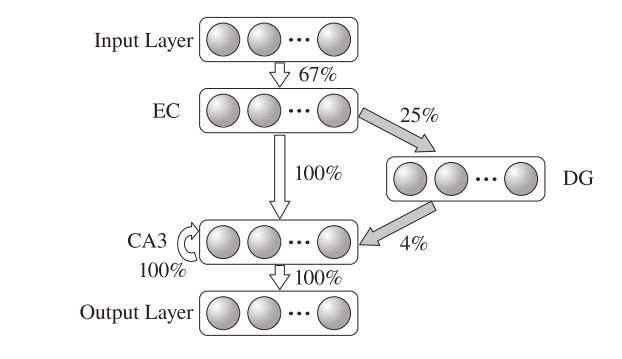
\includegraphics[width=10cm]{fig/hattori2014_hpc_module}
\caption{This figure by \cite{Hattori2014} illustrates his proposed dual-network memory model. Note that the EC is connected to both CA3 and DG, which in turn is also connected to CA3. The gray arrows are connections which are only used during training. Furthermore, CA3 is fully connected both recurrently as well as to the output layer. As EC is connected somewhat sparsely to the DG, and DG is very sparsely connected to CA3, this may constitute a form of compression mechanism as seen in auto-encoders. It is also worth noting that this poses a time-delay from when a certain input has been directly presented from the EC to CA3 until the possibly compressed input arrives from the DG. This may further constitute mechanisms similar to those of operating at multiple timescales, as well as mechanisms for abstraction.}
\label{fig:hattori_2014_model}
\end{figure}

It is worth mentioning that a slightly different transfer function is used by \cite{Hattori2014}. Namely,

\begin{center}
    $f(\theta) = tanh(\frac{\theta}{\epsilon})$,
\end{center}
where $\epsilon$ still is a steepness parameter.

Hebbian learning is still used as in equation \ref{hattori_hebbian_learning} for the CA3-layer and the CA3 to output-layer, relative to its former output;

\begin{center}
\begin{math}
    \omega_{i,j}(t+1) = \gamma \omega_{i,j}(t) + u_i u_j
\end{math}
\end{center}

However, between the EC and DG, EC and CA3, and DG and CA3 parts, Oja's rule is used (\cite{Hertz1991}, cited in \cite{Hattori2014}). Oja's learning rule is a modified type of Hebbian learning, restricting the weight space (to prevent divergence as a result of the chaotic behaviour). It may be formally outlined as follows,

\begin{equation}\label{ojas_rule}
    \omega_{i,j} = \omega_{i,j}(t) + \lambda u_j (u_i - u_j \omega_{i,j}(t)),
\end{equation}
where $\lambda$ is the learning rate for the Oja neurons. Note that the input and output layer neurons are bipolar ($\pm 1$), whereas the other neurons are binary. Every region is trained by a k-winners-take-all (kWTA) approach, in which a fixed number of the $k$ most active neurons' activation values are propagated throughout the neurons' synapses. Neuronal activity is determined by firing frequency. Interestingly, \citep{Hattori2014} notes that the non-linear separation of kWTA seems to be far more powerful than that of non-linear transfer functions. Furthermore, he notes that non-linear transfer functions may actually reduce the performance of kWTA.

One of the final keys to attaining a successful dual-network memory model introduced by \cite{Hattori2014} is neuronal turnover. Neuronal turnover is the birth and extinction of a percentage $\beta \%$ of the neurons, here in the DG. Note, however, that while this is believed to occur to a very low degree biologically in the DG, a very high rate of $\beta = 50 \%$ is employed by \cite{Hattori2014}, with turnover after every training set. Possible reasons for this and associated implications, related to plasticity and convergence, is discussed earlier in this section. \cite{Hattori2014} further demonstrates that the input patterns become less similar when introducing the neuronal turnover, which in turn drastically increases the number of patterns that may be stored in the HPC module.

Memory recall may be performed in the hippocampal network by chaotic recall after learning, i.e. presenting random input to the different sub-networks, waiting until it reaches some convergence criterion, considering the current pattern as a recalled memory. Another approach for interleaving new memories with old, as proposed by \cite{French1997}, is by re-instantiating the previously learned patterns from the neocortical module to the hippocampal network, thus interleaving everything contained in the neocortical network with a new hippocampal pattern. While biologically implausible and not that relevant for the current approach as outlined here, it is worth noting that a similar mechanism for re-instantiated a previously learned pattern to the hippocampal network if present in the neocortical network, might result in attaining novel abstract representations. This could resemble integration across memories more closely, and it is something I wish to further investigate in my future work.


% ======================================================================================

\section{Recurrent Neural Networks}

recurrency in neural networks is simply a directed cycle being present in a network. The simplest form of recurrency is perhaps when a neuron is connected to itself - in other words; recurrently connected. This enables the neuron to 'remember' its former value to a certain extent, combining it with its other current input. Furthermore, more complex recurrencies in networks may enable temporally extended correlations to be captured. An example is the well-known Hopfield network, which exhibits a type of short-term memory. That is, when presented with part of a previously learned pattern, the network will converge towards a steady state consisting of the learned pattern. See figure \ref{fig:hopfield_net} for an illustration of a Hopfield network.

\begin{figure}
\centering
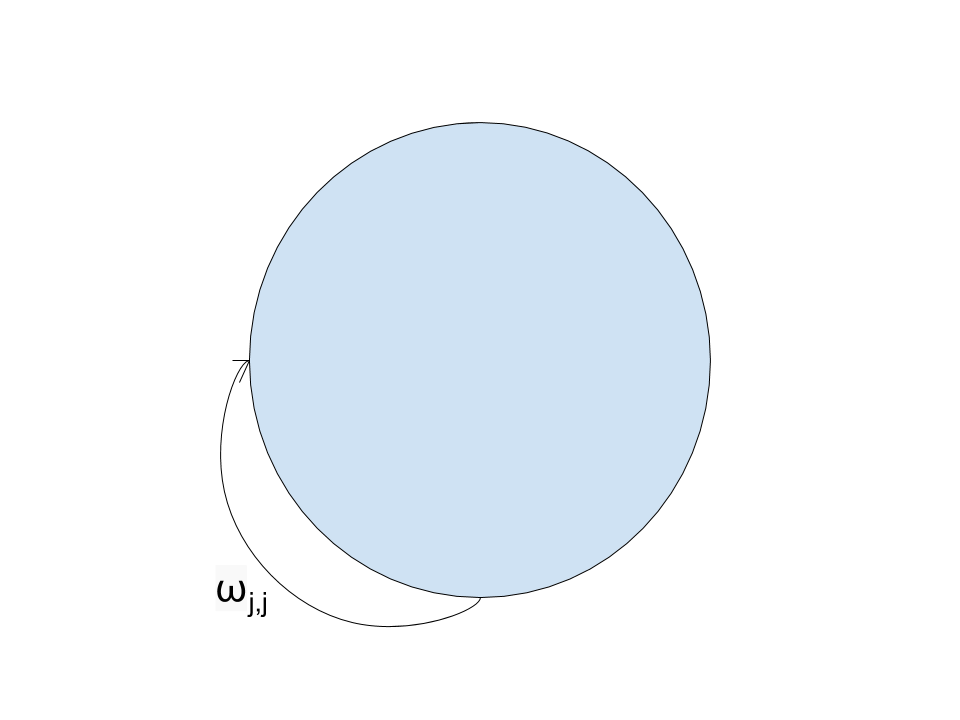
\includegraphics[width=5cm]{fig/one_recurrent_neuron}
\caption{One recurrently connected neuron. This enables a type of short-term memory, potentially capturing small-scale temporal relationships in a recurrent neural network.}
\label{fig:one_recurrent_neuron}
\end{figure}

\begin{figure}
\centering
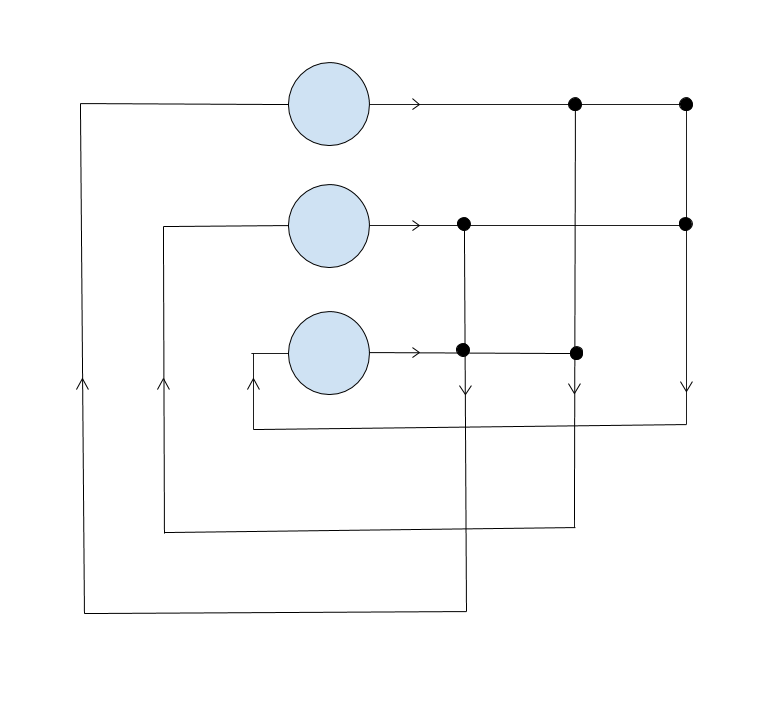
\includegraphics[width=10cm]{fig/hopfield_net}
\caption{Illustrating a simple Hopfield network - a recurrently connected neural network, consisting of three neurons. Activation values flow through the synapses back to all other neurons. This way a neuron may learn its part of a pattern, resulting in partial pattern completion if all other nodes are correctly set. Furthermore, if few patterns relative to the number of neurons are learned, the pattern completion will be more robust, requiring less  information for pattern completion. Note that transfer functions are necessary in this type of network if activation values are propagated without reduction through all synapses.}
\label{fig:hopfield_net}
\end{figure}

In his master's thesis, \cite{Solbakken2009} demonstrates that oscillations between populations of spiking neurons in an RNN model can synchronise the activity of the network as a whole, as well as its sub-networks. This enables the segmentation of multidimensional data through modulatory feedback, also largely avoiding a superposition catastrophe. Namely where objects that are to be segmented share many similar features, and therefore fails to segment them into different categories. With slightly richer neuronal dynamics than what is commonly used, they employ Izhikevich neurons \citep{Izhikevich2003}, attaining a simple model that manages to capture the dynamics of successful segmentation of complex scenes with static input. From this the authors conclude that such a model extends traditional ANNs in including temporal information, in which there is a competitive segmentation process that may separate features, also evading a combinatorial explosion due to the model's dynamics. However, it is unclear which information processing capabilities that emerge by introducing synchronization, and which capabilities emerge implicitly through introducing the Izhikevich neuron model. When it comes to the convergence towards a steady state for a feature that a neural population recognizes: This may potentially provide for richer dynamics in artificial neural networks. Furthermore, evading a combinatorial growth in embedding steady state dynamics in the network could drastically improve deep learning algorithms using deep neural networks. Another concept that \cite{Solbakken2009} addresses in his thesis is the binding problem. As illuminated in his thesis, analogously to how water droplets may condense from steam,  there has to be a change which links meaning to activity in a network model (\cite{Freeman2003}, cited in \cite{Solbakken2009}). A possible coupling between populations of neurons to other populations of neurons is suggested in this regard. It remains obscure, however, how this translates into meaning other than possibly constituting a mechanism for abstraction. Nevertheless, oscillatory dynamics may have the potential to solve several fundamental information processing problems related to neural networks, including memory and segmentation. Therefore, I wish to investigate recurrency and spiking neuron dynamics in my future work in a dual-network memory model.

\cite{Maniadakis2012} demonstrated the ability of recurrent neural networks (RNNs) to self-organize when being evolved by genetic algorithms. They successfully evolved networks which learned a dynamically changing task, navigating in a simulated physical robot environment. Learning such complex behaviour is usually associated with higher order cognitive functions, suggesting that the presented model may relate to the workings of the brain, and more specifically the mechanisms of the prefrontal cortex.
Their study was conducted by using the Wisconsin Card Sorting Test, embedded by a betting function, performed by a robot in a control environment. Because of the nature of the problem domain, and the complexity of the RNNs, they divided the experiment into several phases, in order to better investigate the emergence of network and model properties. Their main findings include that a bottle-neck in the continuous time recurrent neural network architecture was favourable, or even a necessity, in order to attain satisfactory high-level cognitive behaviour. Note that their experiments were limited to very similar environments. Therefore it would be interesting to study the generalisation to differing domains. Note that the paper differs from others in the field in that it regards cognition as embodied both in the model and the environment. As \cite{Bar-yam1997} points out; a complex system is in synthesis with its environment, making it crucial to include the environmental influence on a complex network model when investigating it. It would be interesting to investigate environmental correlates between network topology and network dynamics in future work. Both with respect to a dynamic environment, and with respect to model evolution.

% ====================================
\subsection{Training RNNs}

As one might guess, a fully connected RNN may exhibit cyclic firing patterns, thus constituting a steady-state. This type of dynamics complicates the learning process, making gradient descent as elaborated on in section \ref{BP} a poor candidate for both fully connected recurrent networks, as well as other types of recurrent networks. \cite{Bengio2013b} explains that while gradient-based optimization such as gradient-descent may be used to train RNNs, it generally fails to capture temporal dependencies, especially long-term dependencies. One way of alleviating the problem is by having the recurrent units of an RNN change more slowly, lowering the likelihood for an explosive gradient in certain areas. This is in fact why the field of deep learning has seen a tremendous increase in performance in recent years: long short-term memory (LSTM) units, and gated recurrent units (GRUs) are artificial neurons which enable RNNs to capture long-term temporal dependencies whilst keeping gradient-descent methods as suitable training algorithms. This enabled networks to capture a vast amount of new dependencies, still employing the run-time efficacy and scientific body of insights of gradient-based methods. See section \ref{GRU} (GRUs) for an outline of GRUs.

% ====================================
\subsection{The Gated Recurrent Unit}\label{GRU}

\cite{Cho2014} proposes a novel ANN unit for statistical machine translation using the auto-encoder approach for two RNNs. In their paper the unit was only termed a hidden unit, but as it has later been termed the gated recurrent unit (GRU), this is what I will refer to the unit as throughout this thesis. The GRU is largely inspired by the LSTM, and appears to implement the same behaviour as the LSTM. Therefore I have only chosen to include the formal background for the GRU. As proposed by \cite{Cho2014}, the GRU may be defined formally as follows,

\begin{equation}
    r_j = \sigma ([\textbf{W}_r \textbf{x}]_j + [\textbf{U}_r\textbf{h}_{<t-1>}]_j), 
\end{equation}
where $\sigma$ is the sigmoid function, $\textbf{W}$ are the weights for the input layer $\textbf{x}$, and $\textbf{U}$ are the input weights for the hidden layer $\textbf{h}$.

Furthermore, \cite{Cho2014} defines the update gate $z_j$ as,

\begin{equation}
    z_j = \sigma([\textbf{W}_z\textbf{x}]_j + [\textbf{U}\textbf{h}_{<t-1>}]_j)
\end{equation}
 
With the activation of a hidden state $h_j$ as,
 
\begin{equation}
    h_j^{<t>} = z_j h_j^{<t-1>} + (1 - z_j) \tilde{h}_j^{<t>},
\end{equation}
 
defining,
 
\begin{equation}
    \tilde{h}_j^{<t>} = \phi ([\textbf{W}\textbf{x}]_j + [\textbf{U}(\textbf{r} \odot \textbf{h}_{<t-1>})]_j)
\end{equation}

\begin{figure}
\centering
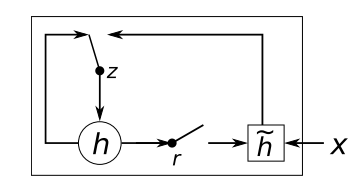
\includegraphics{fig/cho_gru}
\caption{\cite{Cho2014} illustrates their proposed hidden unit, later termed the gated recurrent unit. As outlined in the euqations of \cite{Cho2014} above, the GRU determines whether a hidden state should be updated, and ignored through $z$, and $r$, respectively.}
\label{fig:cho_gru}
\end{figure}

The formulae proposed by \cite{Cho2014}, here presented above, effectively lets an RNN capture long-term temporal dependencies through the correct parametrization of the proposed GRU. Furthermore, a gradient-based approach may be used for optimizing the model weights (\cite{Cho2014}).


% ====================================
\subsection{Multiple-timescales recurrent neural networks}

Functional hierarchies of reusable neural patterns of activation are believed to constitute the mechanisms for among other things motor primitives in the brain. Such functional hierarchies have earlier been realized in artificial neural networks by the explicit coding of hierarchical structure. In this paper, however, \cite{Yamashita2008} propose a novel model in which such a functional hierarchy self-organizes due to the existence of multiple timescales within the network. Thus, the topological split is in a way transformed to a temporal separation, yet now enabling the coordination and segmentation to occur in a more generalisable manner as the reusable motor primitives are no longer hardwired by topological constraints. Their findings still demonstrate that performance is better with a topology supporting segmentation (with a type of bottle-neck between the networks of neurons that operate on different timescales), though segmentation is possible in both cases due to multiple timescales. These findings suggest that there are both spatial and temporal mechanisms which lead to the emergence of functional hierarchies within neural networks. Training is performed by the use of back-propagation through time, in which the desired output generates an error signal. It would be interesting to see what kind of implications different transfer functions would have (with a sigmoid transfer function being used in the proposed model). Furthermore, always enabling a level of training could provide for a more dynamically suitable network. In such an event, the mechanisms for propagation would most likely have to be changed.

\cite{Tani2014} further investigates high-level cognition in neural networks, addressing the key concept of compositionality and how this might constitute cognition. Reviewing evidence suggesting that the mammalian brain attains complex high-level cognition through a functional hierarchy (\cite{Miyake2000, Koechlin2003, Fuster2008}, cited in \cite{Tani2014}), \cite{Tani2014} seeks to gain further knowledge about how this may be constituted at the neural level. Tani introduces two RNN models, and applies each architecture to two different complex tasks, respectively. Both models share the feature of having a type of top-down bottom-up synthesis. In the first architecture using an RNN with a parametric bias (PB) connecting the networks, the top level can be regarded as constantly trying to predict what the lower level is perceiving. If something "unknown" is then perceived, this is learned by a learning mechanism which works on minimizing an error criteria. In the other model, he introduces a multi-network CTRNN architecture, which performs iterative learning on the continuous flow of perceived input. Both models were successfully applied in four different experiments. The main findings include a successful extraction of linguistic properties of sentences and correlated actions and objects with the RNNPB model in the first and second experiment. In the third experiment, the MTRNN successfully attained a functional hierarchy of action primitives, allowing the model to perform complex motor-sensory tasks in a top-down bottom-up synthesis of the higher and lower levels of the MTRNN. A very interesting aspect of the MTRNN is the use of different timescales, with the slower high-level parts of the network enabling this synthesis. Note that this can be regarded as a solution to the symbol grounding problem; the motor-sensory input being a continuous flow of information from the environment, provided by sensory organs, with the symbols and the conscious arising in the synthesis of the functional hierarchy. \cite{Tani2014} contemplates of consciousness as arising in the top-down error minimization-process. This would be in action selection for the case of motor control. Analogously, such a functional hierarchy could be valid for any type of sensory input stream, giving rise to consciousness. In such a hypothesized scenario, the question remains how this could be topologically solved. After all, one of the brain's seemingly central properties is its distributedness and completely decentralized workings. I am inspired in my thesis by the work of \cite{Tani2014} in that I seek to implement principles giving rise to abstraction mechanisms in the dual-network memory architecture of among others \cite{Hattori2014}.

\cite{Tani2014} investigates the emergence of a functional hierarchy of motor primitives in a multiple-timescales recurrent neural network (MTRNN). It consists of two continuous timescale recurrent neural networks (CTRNNs) as sub-networks, each operating at a different timescale. See figure \ref{fig:tani_2014_mtrnn} for an illustration of the structure which \cite{Tani2014} proposes.

\begin{figure}
\centering
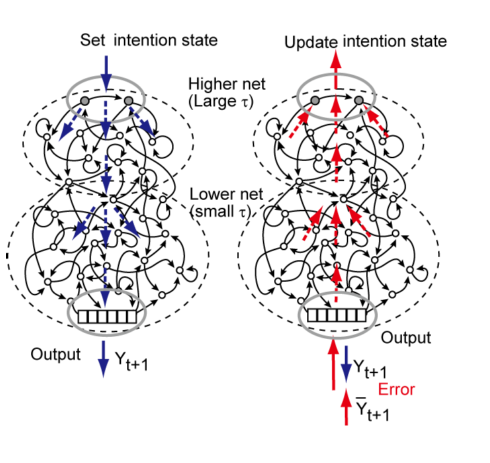
\includegraphics[width=8cm]{fig/tani_2014_mtrnn}
\caption{An illustration by \cite{Tani2014}, in which he illustrates the FFBP process in the proposed MTRNN.}
\label{fig:tani_2014_mtrnn}
\end{figure}

Formally, \cite{Tani2014} proposes the following neural dynamics,

\begin{equation}\label{tani_membrane_potential}
    \tau_i\dot{u}_i = -u_i + \sum_{j}{}\omega_{i,j}a_j + \sum_{k}{}\omega_{i,k} I_k,
\end{equation}

where $\tau_i$ is the time constant, $u_i$ is the membrane potential, $a_i$ is the neural activation state for an internal unit, $y_i$ is the neural activation state for an output unit, and $b_i$ is a bias unit, the subscript denoting a neuron $i$. $\dot{u}_i = \frac{d}{d t}u_i$.

Internal neurons use a sigmoidal transfer function, with the sum of the activation and bias values as input, 

\begin{center}\begin{math}
    a_i = \frac{1}{1+e^{-(u_i+b_i)}},
\end{math}\end{center}
whereas the output neurons use a softmax function,

\begin{equation}\label{tani_softmax}
    y_i = \frac{e^{u_i}}{\sum_{j \in Out}^{}{e^{u_j}}},
\end{equation}
Note that this leads to a fairly sparse representation, where $\sum_{i=1}^{K} y_i = 1$.

In order to train an MTRNN, \cite{Tani2014} defines the Kullback-Leibler divergence as the error criteria $E$ which is to be minimised in order to obtain gradients for weight updates. He then proceeds to derive a formula for recursively calculating $\frac{\partial E}{\partial u_{i,t}}$, which is very similar to a discrete time version of BPTT, and shows that it in fact becomes the discrete BPTT for a certain parameter setting ($\tau=1$). The resulting equations are as follows:

\begin{equation}\label{Kullback_Leibler_divergence}
    E = \sum_t \sum_{i \in Out} y_{i,t}^* log(\frac{y_{i,t}^*}{y_{i,t}}),
\end{equation}
where $y_{i,t}^*$ is the target output and $y_{i,t}$ is the current output for neuron $i$ at time $t$.

\begin{equation}
    \omega_{i,j}(n+1) = \omega_{i,j}(n) - \alpha\frac{\partial E}{\partial \omega_{i,j}},
\end{equation}
where $n$ is the $n$-th iteration step during learning.

\begin{equation}
    \frac{\partial E}{\partial \omega_{i,j}} = \sum_{t} \frac{1}{\tau_i}\frac{\partial E}{\partial u_{i,t}a_{j,t-1}},
\end{equation}
where

\begin{equation}
    \frac{\partial E}{\partial u_{i,t}} = \begin{cases}
        y_{i,t} - y_{i,t}^* + (1-\frac{1}{\tau_i} \frac{\partial E}{\partial u_{i,t+1}}), \text{if $i \in Out$} \\
        \sum_{k \in N}\frac{\partial E}{\partial u_{k,t+1}}[\delta_{i,k}(1-\frac{1}{\tau_i})+\frac{1}{\tau_k}\omega_{k,i}f'(u_{i,t})], \text{if $\notin Out$}
   \end{cases}
\end{equation}
where $\delta$ is the Kronecker Delta function, i.e.,

\begin{center}
\begin{math}
    \delta = \begin{cases}
        0, \text{if $i \neq k$} \\
        1, \text{if $i = k$}
    \end{cases}
\end{math}
\end{center}

The MTRNN improves the PB-vector approach, where the synchronization of two modules that extract the 'knowledge' to perform two distinct tasks occurs. I find this very interesting (and intriguing) in terms of the self-organization of a functional hierarchy, and I wish to investigate the potential applicability of this approach in the dual-network memory architecture in my future work. For instance whether it would be possible to use an MTRNN to extract a functional hierarchy that may be consolidated to the neocortical network. This could have potential implications for re-instantiation of previously learned functionality from the neocortical network into the hippocampal network. Another aspect that is worth emphasizing is that it could possibly enable the neocortical network to organize its memories in a more meaningful and coherent way.

\section{Summary}

The topics of this thesis are abstraction, catastrophic forgetting and generalisation in artificial neural networks. The dual-network memory architecture \citep{McClelland1995, French1997, Ans1997, Hattori2014} seems to form a suitable architecture for further investigation of these aspects in ANNs. Furthermore, novel state-of-the-art techniques such as using GRUs in RNNs have enabled algorithms to capture long-term temporal dependencies, whilst still remaining suitable for training with gradient-based methods. This might be employed in a neocortical network in a novel dual-network memory model. Another problem which is tightly coupled to memory formation and abstraction is the self-organization of a functional hierarchy in ANNs, which has been realized using MTRNNs in \citep{Yamashita2008, Tani2014}. I wish to extend the dual-network memory architecture by implementing GRUs in the neocortical module, and to investigate the potential of further model extensions using MTRNNs.


\cleardoublepage